\clearpage\subsection*{1−5 ポート番号とは}
\refstepcounter{PagePtr}\label{P:port}

\centering
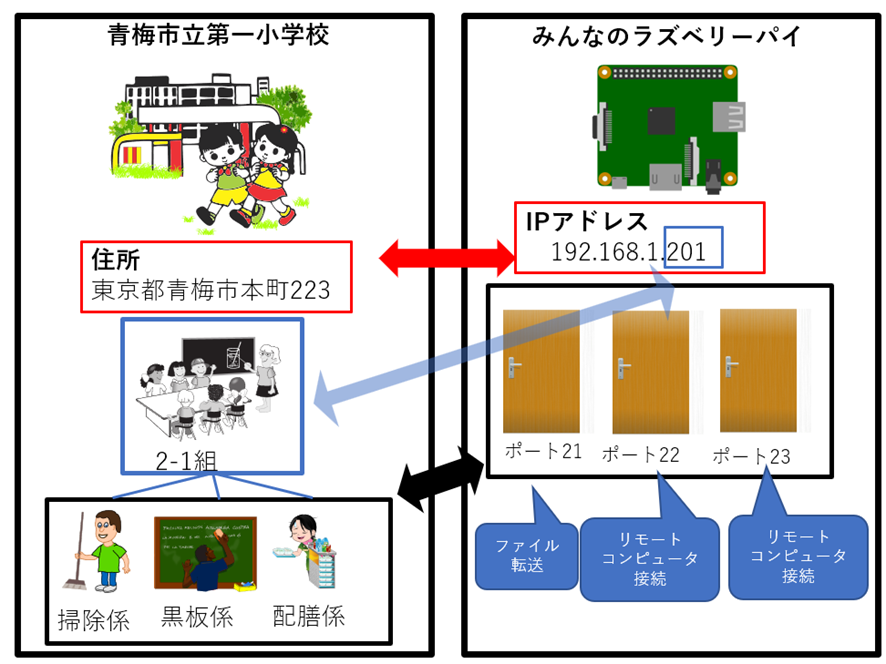
\includegraphics[width=0.85\textwidth]{ome7-img020.png}
\flushleft

前のページではみんなはラズベリーパイがどのようにインターネットにつながっているのか理解してくれたと思います。
ここではさらにポート番号について\ruby{知識}{ちしき}を深めましょう。
IPアドレスでは通信相手となる別のネットワークのコンピュータを特定することができます。
しかし、コンピュータでは\ruby{通常}{つうじょう}、多くのプログラム(機能)が動作していて、IPアドレスを指定するだけでは、どのプログラムと接続するかを区別できません。
そこでコンピュータ上の、\underline{どのプログラムと接続するかを指定するためにポート番号が用いられます}。
下の図は小学校を例にしています。

青梅市立第一小学校の住所がみんなのラズベリーパイのIPアドレスに\ruby{対応}{たいおう}しており、IPアドレスの\ruby{末尾}{まつび}の201(青で囲まれている)が小学校のクラスに対応しています。
皆さんの学校でも生徒にはそれぞれ係という役割が\ruby{与}{あた}えられていますね。
例えば、プリントなどの\ruby{配布物}{はいふぶつ}を配る配り係、黒板を使い終わったらきれいにする黒板係、教室の\ruby{窓}{まど}をきれいにする窓ふき係などこれらの係に相当するものがラズベリーパイにもあり、それが\underline{ポート}です。
ポート21はファイル転送用の働きをする\ruby{担当}{たんとう}で、ポート22と23は他のコンピュータに接続する担当です。
ポートには役割がありインターネットの通信はファイル転送であったり、他のコンピュータに接続して\ruby{遠隔}{えんかく}操作したり、webページにアクセスしたりといろいろあります。
なので、その分のポートを用意しておき、役割を与え、対応している役割のときに\ruby{頑張}{がんば}ってもらう仕組みになっています。
みんなのラズベリーパイやパソコン、サーバにはポートは何個あるのか調べてみるのも面白いですね。

\clearpage
\refstepcounter{Question}\theQuestion ポート番号はどのようなことに使われますか。\label{Q:portUsage}

\addBlank{答え}

ここでは実際にポートはネットワーク上ではどのように使うのか、下の図を見てみましょう。

\centering
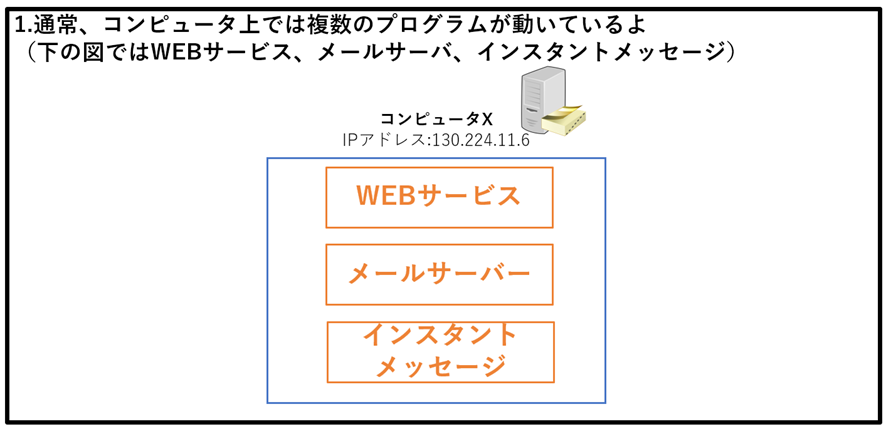
\includegraphics[width=0.97\textwidth]{ome7-img021.png}

\centering
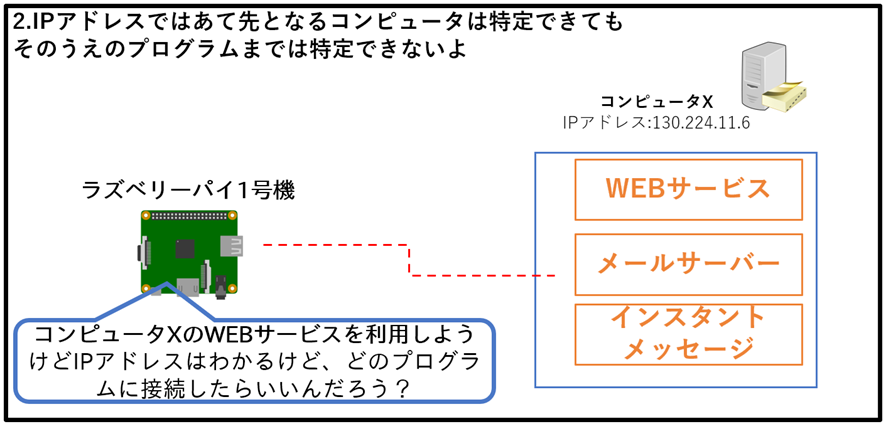
\includegraphics[width=0.97\textwidth]{ome7-img022.png}
\flushleft


\clearpage

\centering
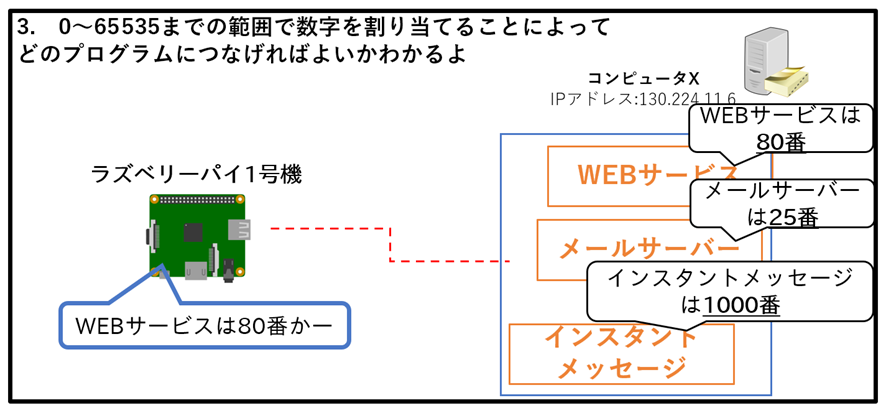
\includegraphics[width=0.97\textwidth]{ome7-img023.png}

\centering
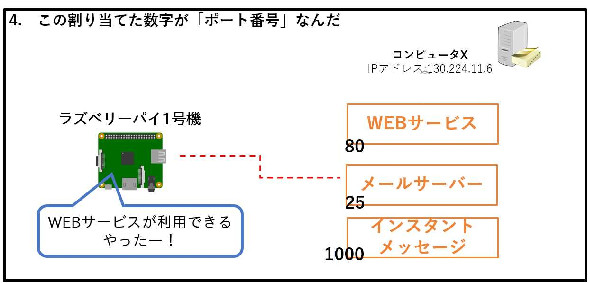
\includegraphics[width=0.97\textwidth]{ome7-img024}
\flushleft

さらにラズベリーパイ側のポートはラズベリーパイが自動で割当ており、そこからデータを受け取っているよ。

\centering
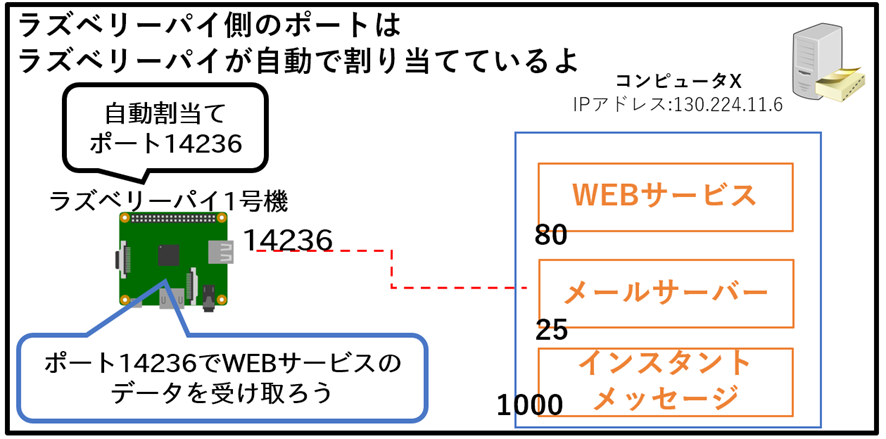
\includegraphics[width=0.97\textwidth]{ome7-img025.png}
\flushleft

コンピュータXのようにネット上にサービスを\ruby{提供}{ていきょう}するコンピュータを\underline{サーバ}と言います。

ラズベリーパイ1号機のようにサーバからサービスを受けるコンピュータを\underline{クライアント}言います。

これらのポートが今\ruby{現在}{げんざい}どのようなことに使われているのか\textbf{\ref{port}で確認してみましょう。}

{\refstepcounter{Question}\theQuestion コンピュータ上のプログラムを判断するためになにが用いられていますか。\label{Q:port}}

{\bfseries \addBlank{答え}}

{\bfseries ネット上にサービスを提供するコンピュータとネット上のコンピュータからサービスを受けるコンピュータをそれぞれ何といいますか。}

{\bfseries \addBlank{答え}}

\clearpage
\subsection*{1−6 DNS(Domain Name System)について}
\refstepcounter{PagePtr}\label{P:DNS}

{\bfseries IPアドレスは住所であり、それがわからないとサーバのサービスをうけることはできません。ですが以下の図のようなことが起こることがあります。}

\centering
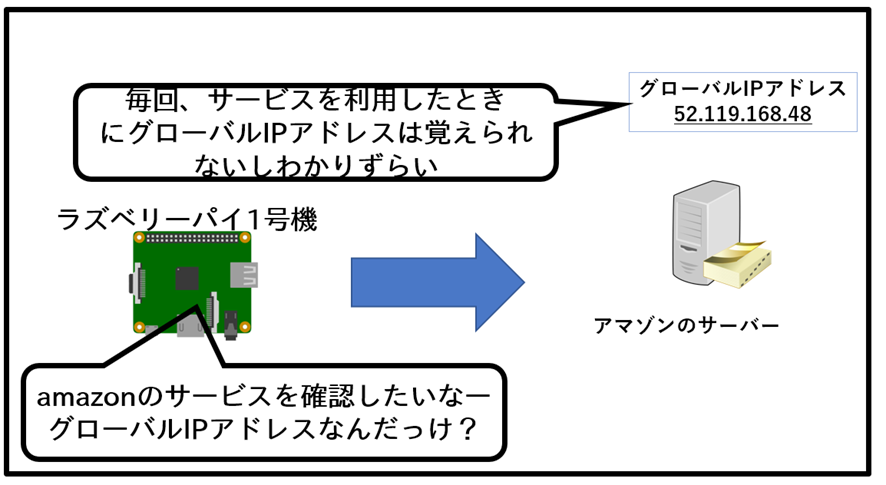
\includegraphics[width=0.97\textwidth]{ome7-img026.png}
\flushleft

そこで、DNSサーバと言うものを作り、一度そこに”amazon.co.jp”のグローバルIPアドレスを教えてもらってサーバに接続しています。

\centering
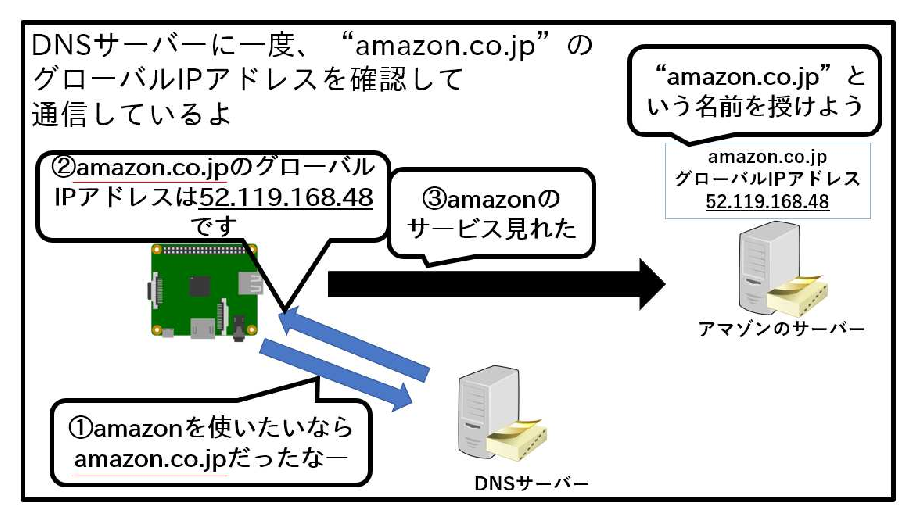
\includegraphics[width=0.97\textwidth]{ome7-img027}
\flushleft

\clearpage

\centering
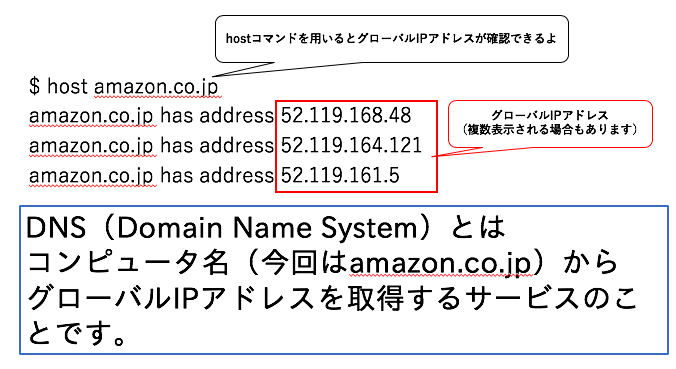
\includegraphics[width=0.8\textwidth]{ome7-img028.png}
\flushleft

{\refstepcounter{Question}\theQuestion ターミナルを開き、”dig amazon.co.jp”を実行してグローバルIPアドレスを確認しよう。\label{Q:dig}}

{\bfseries \addBlank{答え}}

\clearpage
\subsection*{\bfseries コラム NATについて}

教科書の前のページでローカルIPアドレスとグローバルIPアドレスが存在することを皆さんは知りましたね。ここではもっと細かくIPアドレスを用いたインターネット接続を勉強しましょう。インターネットに接続するコンピュータは自分自身を示すIPアドレスとして世界で\ruby{唯一}{ゆいつ}のグローバルIPアドレスを使わなければならないのです。みなさんのラズベリーパイにはローカルIPアドレスしか割り当てられていませんので、このままではインターネットをすることはできません。そこでNAT(Network
Address
Translation)というものを用います。このNATはルータが行っていて、送信元のローカルIPアドレスをグローバルIPアドレスに変換して通信を行っています。具体的にはどのようになっているのか下の図をみて確認してみよう。

\centering
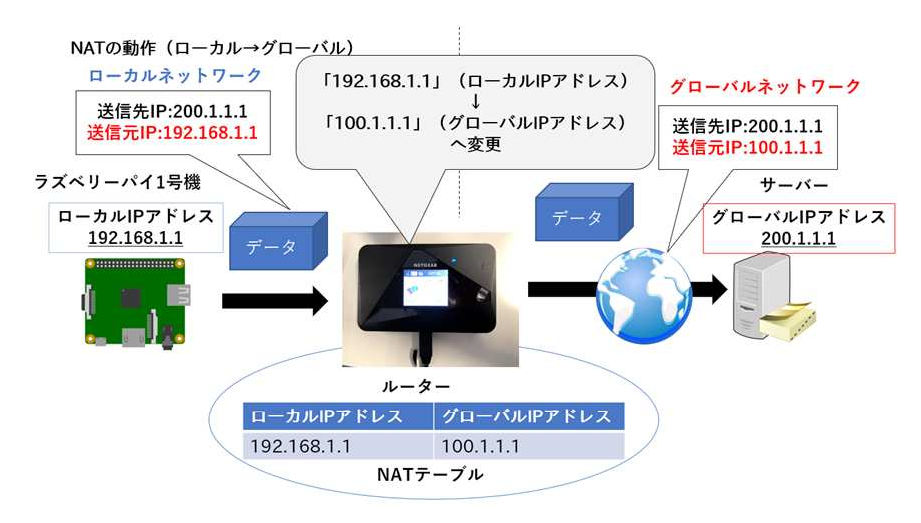
\includegraphics[width=0.9\textwidth]{ome7-img029}
\flushleft

\clearpage
ラズベリーパイ1号機からサーバにデータの送信先IPアドレスは200.1.1.1(グローバルIPアドレス)、送信元IPアドレスは192.168.1.1(ローカルIPアドレス)です。NATを行うルータは、プライベートアドレスとグローバルアドレスの\ruby{境界}{きょうかい}に位置しています。ここでルータは、ラズベリーパイから送信されたデータの送信元IPアドレス192.168.1.1を、グローバルIPアドレスの「100.1.1.1」に変換して転送します。このときルータは、その変換情報をNATテーブルに記録しています。この記録が、「返ってくるデータ」、つまりサーバーからラズベリーパイへ送られるデータの転送時に役立ちます。次の図を見てください。

\centering
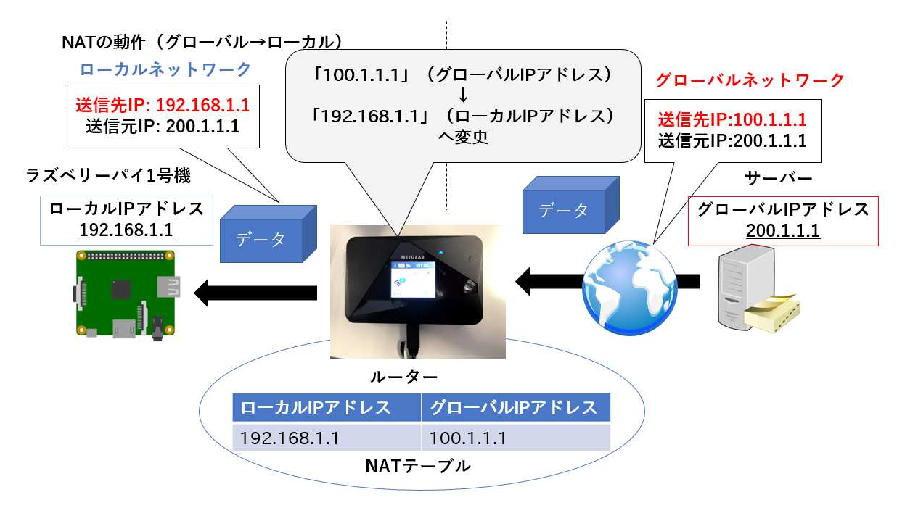
\includegraphics[width=0.9\textwidth]{ome7-img030}
\flushleft

サーバーからラズベリーパイへの返事のデータの送信先IPアドレスは「100.1.1.1」、送信元IPアドレス「200.1.1.1」になりますね。データがルータへ転送されてくると、ルータはNATテーブルを確認して、送信元IPアドレスを「100.1.1.1」から元の「192.168.1.1」へ変換します。これにより返りのデータの通信が可能になるのです。NATによって送信元のローカルIPアドレスをグローバルIPアドレスに変換して通信をおこなっているおかげでみんなはインターネットを利用できているんだね。

\refstepcounter{Exercise}
\clearpage
\subsection*{\theExercise 開いているポートを調べてみよう}
\addtocounter{Exercise}{-1}\refstepcounter{Exercise}\label{port}
ターミナルを開き、”nmap
localhost”とコマンドを入力し、ポートについて知ろう

{\bfseries 方法}

\centering
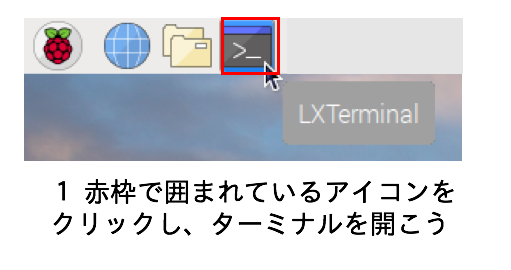
\includegraphics[width=0.85\textwidth]{ome7-img007.png}

\centering
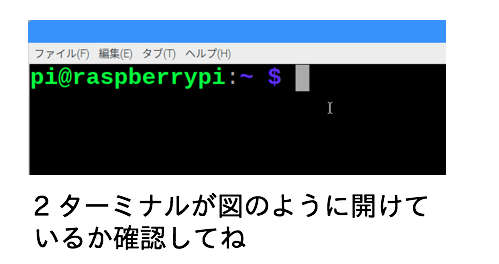
\includegraphics[width=0.85\textwidth]{ome7-img008.png}
\flushleft


\clearpage

\centering
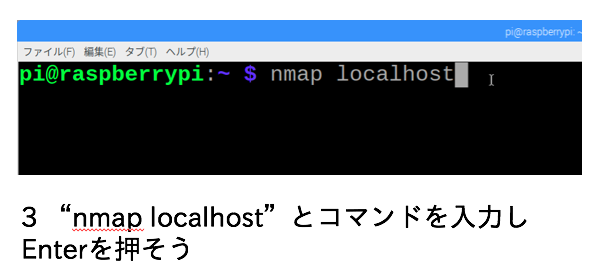
\includegraphics[width=0.85\textwidth]{ome7-img032.png}
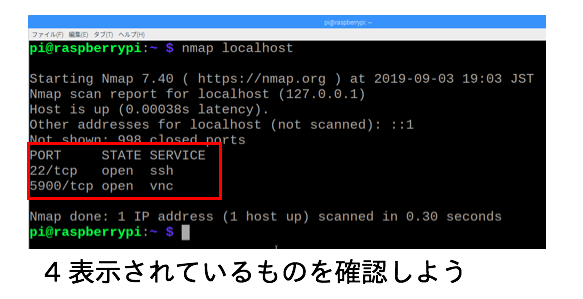
\includegraphics[width=0.85\textwidth]{ome7-img031.png}
\flushleft

{\bfseries 自分のラズベリーパイに表示されたものを下の表に書こう}

\begin{flushleft}
	\tablefirsthead{}
	\tablehead{}
	\tabletail{}
	\tablelasttail{}
	\begin{supertabular}{|m{5.467cm}|m{5.4690003cm}|m{5.155cm}|}
		\hline
		PORT & STATE & SERVICE\\\hline
		~ &	~ & ~ \\\hline
		~ &	~ & ~ \\\hline
		~ &	~ & ~ \\\hline
		~ &	~ & ~ \\\hline
	\end{supertabular}
\end{flushleft}
{\bfseries
serviceに出てきた言葉をインターネットを使って調べよう。
皆さんにとっては\ruby{難}{むず}しい言葉が多いと思います。
それでも自分で調べてみましょう。
それが知識を深める近道です。\\
ポートが開いていない場合、コマンドは何も表示せず、
改行が起こるだけのこともあります。
}
